\part{Search}
\frame{\partpage}

\newcommand{\namesunsorted}{
	\fbox{\parbox{0.9\textwidth}{\tiny
		Anderson, Martha \par
		Parker, Debra \par
		Russell, Mildred \par
		Stewart, Howard \par
		White, Amanda \par
		Perez, Diana \par
		Lewis, Rose \par
		Scott, Michelle \par
		Davis, Marilyn \par
		Cox, Shirley \par
		Young, Frank \par
		Collins, Jane \par
		Kelly, Philip \par
		Miller, Jeremy \par
		Clark, Stephanie \par
		Brown, Janet \par
		Diaz, Harold \par
		Hughes, Aaron \par
		Sanders, Phillip \par
		Williams, Billy \par
		Henderson, Lawrence \par
		Baker, Theresa \par
		Gonzalez, Adam \par
		Lopez, Jeffrey \par
		Ward, Jessica
	}}
}

\newcommand{\namessorted}{
	\fbox{\parbox{0.9\textwidth}{\tiny
		Anderson, Martha \par
		Baker, Theresa \par
		Brown, Janet \par
		Clark, Stephanie \par
		Collins, Jane \par
		Cox, Shirley \par
		Davis, Marilyn \par
		Diaz, Harold \par
		Gonzalez, Adam \par
		Henderson, Lawrence \par
		Hughes, Aaron \par
		Kelly, Philip \par
		Lewis, Rose \par
		Lopez, Jeffrey \par
		Miller, Jeremy \par
		Parker, Debra \par
		Perez, Diana \par
		Russell, Mildred \par
		Sanders, Phillip \par
		Scott, Michelle \par
		Stewart, Howard \par
		Ward, Jessica \par
		White, Amanda \par
		Williams, Billy \par
		Young, Frank
	}}
}

\begin{frame}{Search}
			\begin{itemize}
				\item We have a list of names, each with some data associated \pause
				\item We want to find one of them
			\end{itemize}
\end{frame}

\begin{frame}{Linear search}
			\begin{algorithmic}
				\Procedure{Find}{name, list} \pause
					\For{each item in list} \pause
						\If{item.name $=$ name} \pause
							\State \textbf{return} item \pause
						\EndIf
					\EndFor
					\State \textbf{throw} ``Not found'' \pause
				\EndProcedure
			\end{algorithmic}
\end{frame}

\begin{frame}{How long does it take?}
	Socrative room code: \texttt{FALCOMPED}
	\begin{itemize}
		\item Suppose there are 25 items in the list \pause
		\item In the \textbf{best case}, how many items do we need to visit before finding the one we want? \pause
		\item How about in the \textbf{worst case}?
	\end{itemize}
\end{frame}

\begin{frame}{How long does it take?}
	Socrative room code: \texttt{FALCOMPED}
	\begin{itemize}
		\item If there are 25 items in the list, the \textbf{worst case} number of items visited is 25 \pause
		\item How about if there are 50 items? \pause
		\item How about 100 items? \pause
		\item If the number of items \textbf{doubles}, what happens to the amount of time the search takes?
	\end{itemize}
\end{frame}

\begin{frame}{Linear time}
	\begin{columns}
		\begin{column}{0.45\textwidth}
			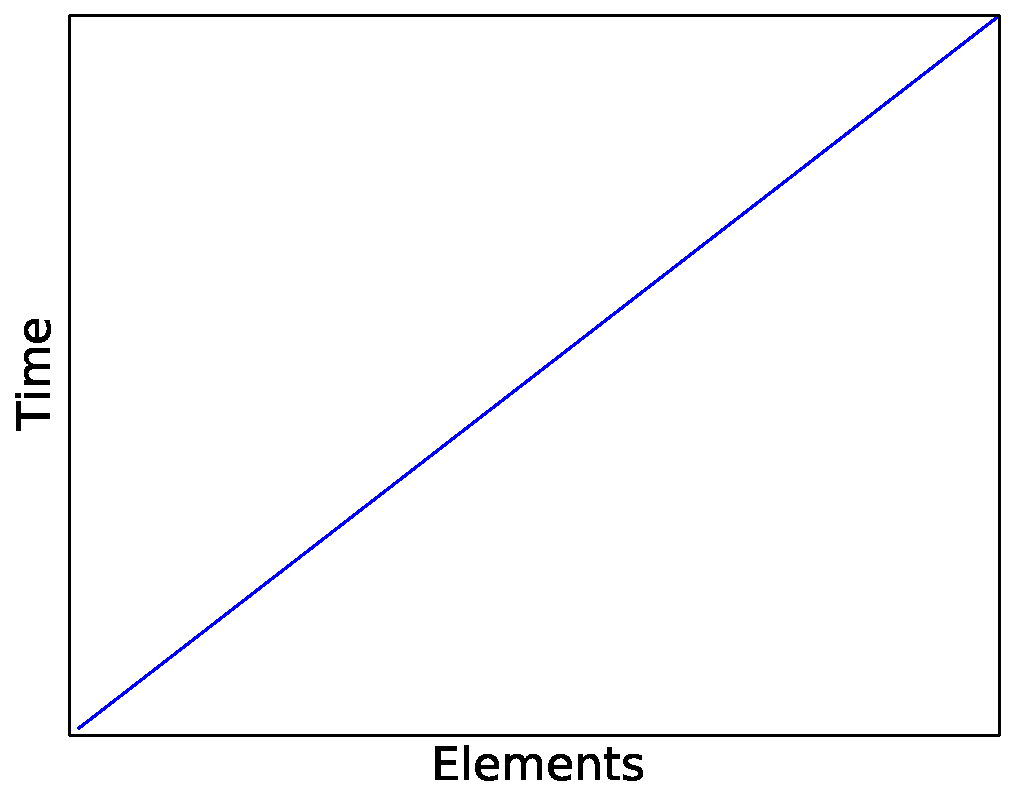
\includegraphics[width=\textwidth]{plot2_linear}
		\end{column}
		\begin{column}{0.55\textwidth}
			\begin{itemize}
				\item The running time of linear search is \textbf{proportional} to the size $n$ of the list \pause
				\item Linear search is said to have \textbf{linear time complexity} \pause
				\item Also written as \textbf{$O(n)$ time complexity}
			\end{itemize}
		\end{column}
	\end{columns}
\end{frame}

\begin{frame}{Searching a sorted list}
			\begin{itemize}
				\item If the list is \textbf{sorted} in alphabetical order, we can do better than linear...
			\end{itemize}
\end{frame}

\begin{frame}{Binary search}
	\begin{algorithmic}
		\Procedure{Find}{name, list} \pause
			\If{list is empty}
				\State \textbf{throw} ``Not found''
			\EndIf \pause
			\State mid $\gets$ the ``middle'' item of the list \pause
			\If{name $=$ mid.name}
				\State \textbf{return} mid \pause
			\ElsIf{name $<$ mid.name}
				\State \textbf{return} \Call{Find}{name, first half of list} \pause
			\ElsIf{name $>$ mid.name}
				\State \textbf{return} \Call{Find}{name, second half of list} \pause
			\EndIf
		\EndProcedure
	\end{algorithmic}
\end{frame}

\begin{frame}{Find ``Lopez, Jeffrey''}
	\begin{columns}
		\begin{column}{0.3\textwidth}
			\fbox{\parbox{0.9\textwidth}{\tiny
				$\phantom\longrightarrow$ Anderson, Martha \par
				$\phantom\longrightarrow$ Baker, Theresa \par
				$\phantom\longrightarrow$ Brown, Janet \par
				$\phantom\longrightarrow$ Clark, Stephanie \par
				$\phantom\longrightarrow$ Collins, Jane \par
				$\phantom\longrightarrow$ Cox, Shirley \par
				$\phantom\longrightarrow$ Davis, Marilyn \par
				$\phantom\longrightarrow$ Diaz, Harold \par
				$\phantom\longrightarrow$ Gonzalez, Adam \par
				$\phantom\longrightarrow$ Henderson, Lawrence \par
				$\phantom\longrightarrow$ Hughes, Aaron \par
				$\phantom\longrightarrow$ Kelly, Philip \par
				$\longrightarrow$ Lewis, Rose \par
				$\phantom\longrightarrow$ Lopez, Jeffrey \par
				$\phantom\longrightarrow$ Miller, Jeremy \par
				$\phantom\longrightarrow$ Parker, Debra \par
				$\phantom\longrightarrow$ Perez, Diana \par
				$\phantom\longrightarrow$ Russell, Mildred \par
				$\phantom\longrightarrow$ Sanders, Phillip \par
				$\phantom\longrightarrow$ Scott, Michelle \par
				$\phantom\longrightarrow$ Stewart, Howard \par
				$\phantom\longrightarrow$ Ward, Jessica \par
				$\phantom\longrightarrow$ White, Amanda \par
				$\phantom\longrightarrow$ Williams, Billy \par
				$\phantom\longrightarrow$ Young, Frank
			}}
		\end{column}
	\end{columns}
\end{frame}

\begin{frame}{Find ``Lopez, Jeffrey''}
	\begin{columns}
		\begin{column}{0.3\textwidth}
			\fbox{\parbox{0.9\textwidth}{\tiny
				{\color{gray}
				$\phantom\longrightarrow$ Anderson, Martha \par
				$\phantom\longrightarrow$ Baker, Theresa \par
				$\phantom\longrightarrow$ Brown, Janet \par
				$\phantom\longrightarrow$ Clark, Stephanie \par
				$\phantom\longrightarrow$ Collins, Jane \par
				$\phantom\longrightarrow$ Cox, Shirley \par
				$\phantom\longrightarrow$ Davis, Marilyn \par
				$\phantom\longrightarrow$ Diaz, Harold \par
				$\phantom\longrightarrow$ Gonzalez, Adam \par
				$\phantom\longrightarrow$ Henderson, Lawrence \par
				$\phantom\longrightarrow$ Hughes, Aaron \par
				$\phantom\longrightarrow$ Kelly, Philip \par
				$\phantom\longrightarrow$ Lewis, Rose \par
				}
				$\phantom\longrightarrow$ Lopez, Jeffrey \par
				$\phantom\longrightarrow$ Miller, Jeremy \par
				$\phantom\longrightarrow$ Parker, Debra \par
				$\phantom\longrightarrow$ Perez, Diana \par
				$\phantom\longrightarrow$ Russell, Mildred \par
				$\longrightarrow$ Sanders, Phillip \par
				$\phantom\longrightarrow$ Scott, Michelle \par
				$\phantom\longrightarrow$ Stewart, Howard \par
				$\phantom\longrightarrow$ Ward, Jessica \par
				$\phantom\longrightarrow$ White, Amanda \par
				$\phantom\longrightarrow$ Williams, Billy \par
				$\phantom\longrightarrow$ Young, Frank
			}}
		\end{column}
	\end{columns}
\end{frame}

\begin{frame}{Find ``Lopez, Jeffrey''}
	\begin{columns}
		\begin{column}{0.3\textwidth}
			\fbox{\parbox{0.9\textwidth}{\tiny
				{\color{gray}
				$\phantom\longrightarrow$ Anderson, Martha \par
				$\phantom\longrightarrow$ Baker, Theresa \par
				$\phantom\longrightarrow$ Brown, Janet \par
				$\phantom\longrightarrow$ Clark, Stephanie \par
				$\phantom\longrightarrow$ Collins, Jane \par
				$\phantom\longrightarrow$ Cox, Shirley \par
				$\phantom\longrightarrow$ Davis, Marilyn \par
				$\phantom\longrightarrow$ Diaz, Harold \par
				$\phantom\longrightarrow$ Gonzalez, Adam \par
				$\phantom\longrightarrow$ Henderson, Lawrence \par
				$\phantom\longrightarrow$ Hughes, Aaron \par
				$\phantom\longrightarrow$ Kelly, Philip \par
				$\phantom\longrightarrow$ Lewis, Rose \par
				}
				$\phantom\longrightarrow$ Lopez, Jeffrey \par
				$\phantom\longrightarrow$ Miller, Jeremy \par
				$\longrightarrow$ Parker, Debra \par
				$\phantom\longrightarrow$ Perez, Diana \par
				$\phantom\longrightarrow$ Russell, Mildred \par
				{\color{gray}$\phantom\longrightarrow$ Sanders, Phillip \par
				$\phantom\longrightarrow$ Scott, Michelle \par
				$\phantom\longrightarrow$ Stewart, Howard \par
				$\phantom\longrightarrow$ Ward, Jessica \par
				$\phantom\longrightarrow$ White, Amanda \par
				$\phantom\longrightarrow$ Williams, Billy \par
				$\phantom\longrightarrow$ Young, Frank
				}
			}}
		\end{column}
	\end{columns}
\end{frame}

\begin{frame}{Find ``Lopez, Jeffrey''}
	\begin{columns}
		\begin{column}{0.3\textwidth}
			\fbox{\parbox{0.9\textwidth}{\tiny
				{\color{gray}
				$\phantom\longrightarrow$ Anderson, Martha \par
				$\phantom\longrightarrow$ Baker, Theresa \par
				$\phantom\longrightarrow$ Brown, Janet \par
				$\phantom\longrightarrow$ Clark, Stephanie \par
				$\phantom\longrightarrow$ Collins, Jane \par
				$\phantom\longrightarrow$ Cox, Shirley \par
				$\phantom\longrightarrow$ Davis, Marilyn \par
				$\phantom\longrightarrow$ Diaz, Harold \par
				$\phantom\longrightarrow$ Gonzalez, Adam \par
				$\phantom\longrightarrow$ Henderson, Lawrence \par
				$\phantom\longrightarrow$ Hughes, Aaron \par
				$\phantom\longrightarrow$ Kelly, Philip \par
				$\phantom\longrightarrow$ Lewis, Rose \par
				}
				$\longrightarrow$ Lopez, Jeffrey \par
				$\phantom\longrightarrow$ Miller, Jeremy \par
				{\color{gray}$\phantom\longrightarrow$ Parker, Debra \par
				$\phantom\longrightarrow$ Perez, Diana \par
				$\phantom\longrightarrow$ Russell, Mildred \par
				$\phantom\longrightarrow$ Sanders, Phillip \par
				$\phantom\longrightarrow$ Scott, Michelle \par
				$\phantom\longrightarrow$ Stewart, Howard \par
				$\phantom\longrightarrow$ Ward, Jessica \par
				$\phantom\longrightarrow$ White, Amanda \par
				$\phantom\longrightarrow$ Williams, Billy \par
				$\phantom\longrightarrow$ Young, Frank
				}
			}}
		\end{column}
	\end{columns}
\end{frame}

\begin{frame}{How long does it take?}
	Socrative room code: \texttt{FALCOMPED}
	\begin{columns}
		\begin{column}{0.55\textwidth}
			\begin{itemize}
				\item Each iteration cuts the list in \textbf{half} \pause
				\item Worst case: we have to keep halving until we get down to a single element \pause
				\item If the size of the list is \textbf{doubled}, what happens to the worst-case
					\textbf{number of iterations} required? \pause
				\iftoggle{printable}{}{\item \textbf{Answer:} it increases by 1 \pause}
				\item The running time is \textbf{logarithmic} or $O(\log n)$ \pause
			\end{itemize}
		\end{column}
		\begin{column}{0.45\textwidth}
			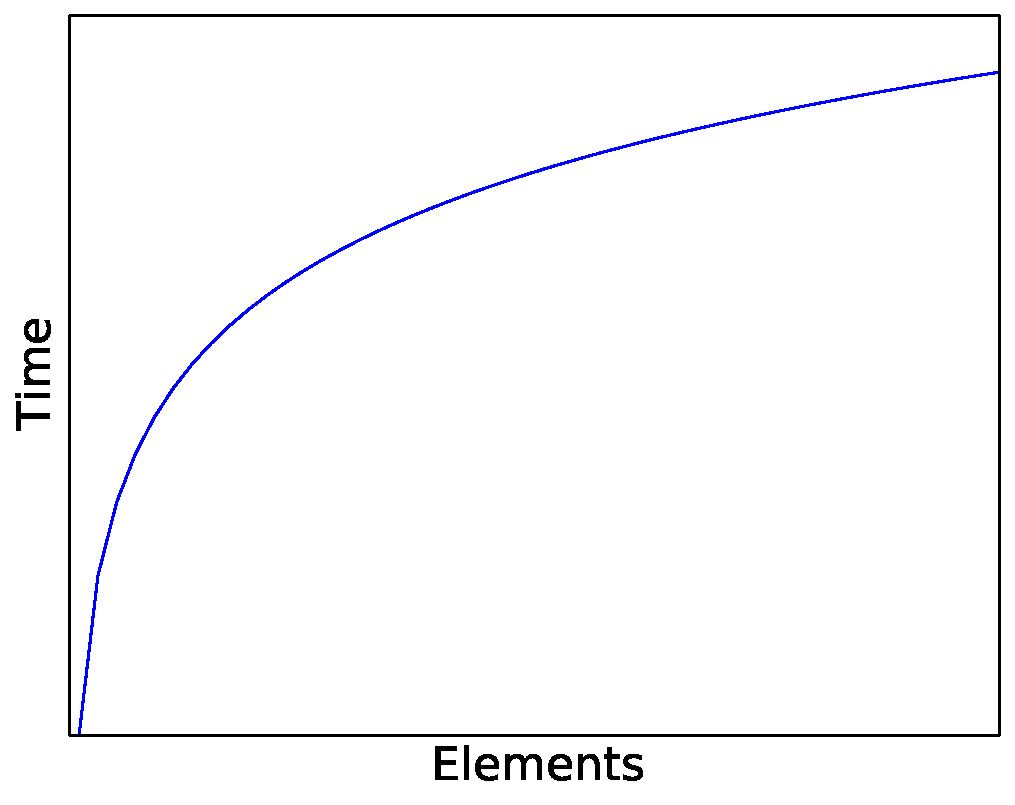
\includegraphics[width=\textwidth]{plot2_log}
		\end{column}
	\end{columns}
\end{frame}

\begin{frame}{Hidden complexity}
	\begin{algorithmic}
			\If{name $<$ mid.name}
				\State \textbf{return} \Call{Find}{name, first half of list}
			\ElsIf{name $>$ mid.name}
				\State \textbf{return} \Call{Find}{name, second half of list}
			\EndIf
	\end{algorithmic}
	\pause
	\begin{columns}
		\begin{column}{0.45\textwidth}
			\only<4->{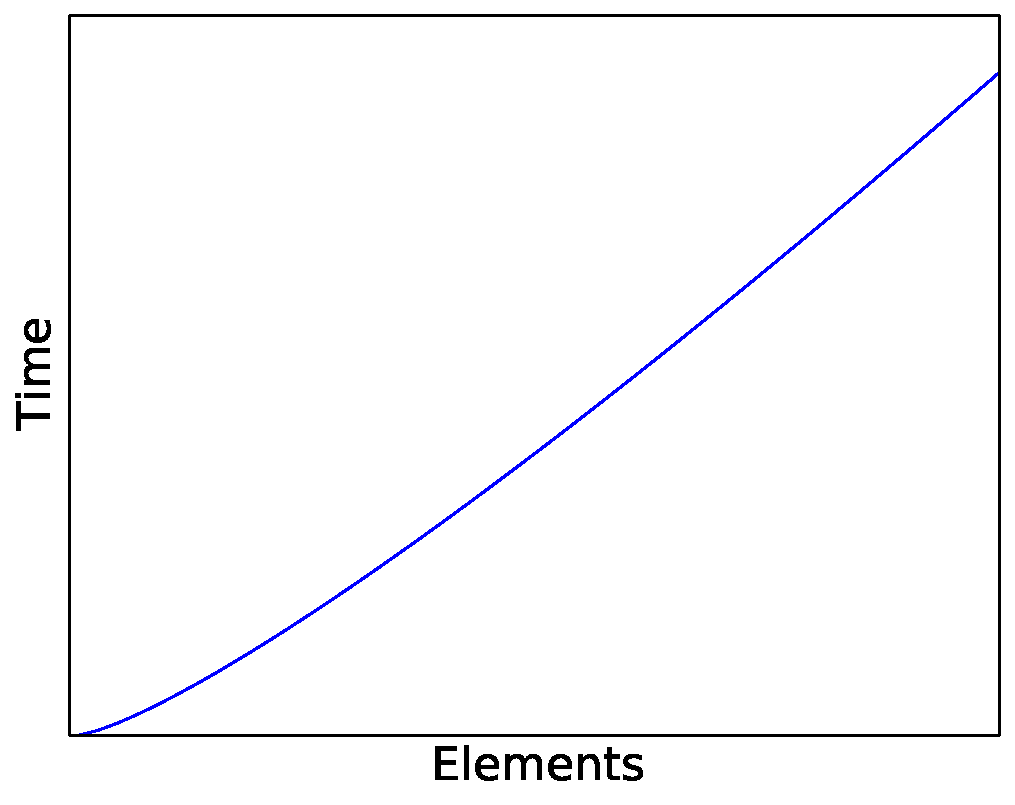
\includegraphics[width=\textwidth]{plot2_nlogn}}
		\end{column}
		\begin{column}{0.55\textwidth}
			\begin{itemize}
				\item Careful how you implement this! \pause
				\item \textbf{Copying} (half of) a list is \textbf{linear} $O(n)$ \pause
				\item The actual running time would be $O(n \log n)$ \pause
				\item Use \textbf{pointers} into the list instead of copying
			\end{itemize}
		\end{column}
	\end{columns}
\end{frame}

\begin{frame}{Binary search done wrong}
	\lstinputlisting[language=Python]{binary_search_bad.py}
\end{frame}

\begin{frame}{Binary search done right}
	\lstinputlisting[language=Python]{binary_search_good.py}
\end{frame}

\begin{frame}{Binary search vs linear search}
	\begin{columns}
		\begin{column}{0.45\textwidth}
			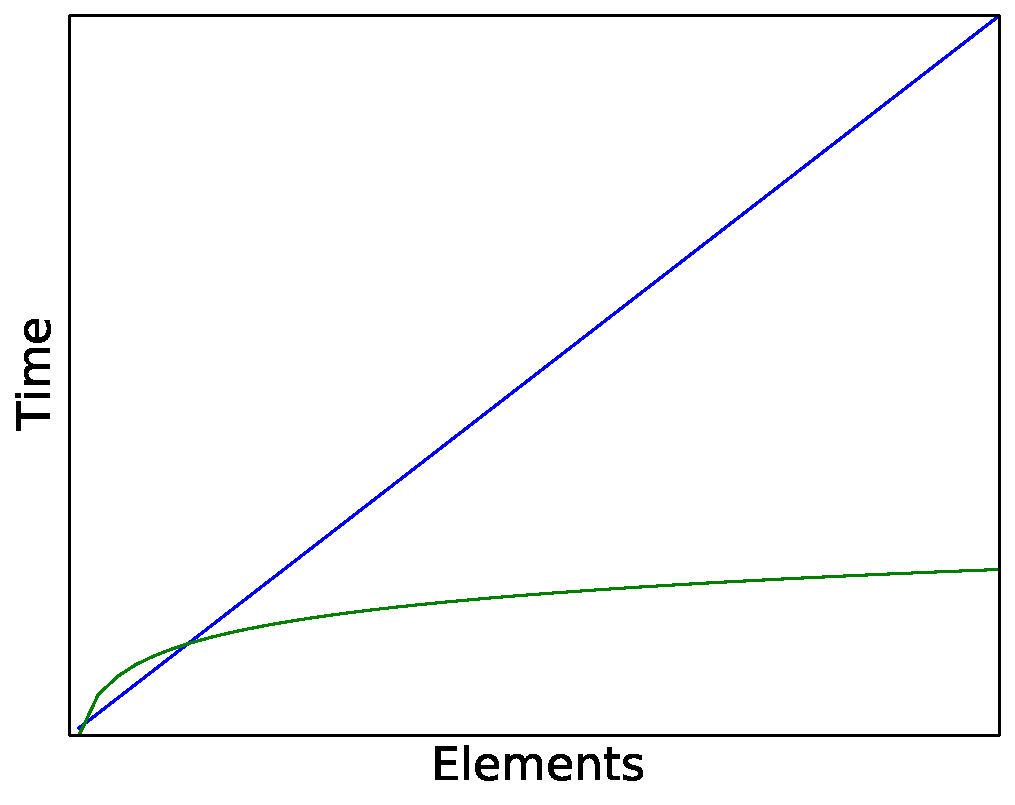
\includegraphics[width=\textwidth]{plot2_linear_log}
		\end{column}
		\begin{column}{0.55\textwidth}
			\begin{itemize}
				\item So binary search is better than linear search... right?
			\end{itemize}
		\end{column}
	\end{columns}
\end{frame}

\begin{frame}{Hashing}
	\begin{columns}
		\begin{column}{0.66\textwidth}
			\begin{itemize}
				\item Come up with a \textbf{hashing function} which maps elements to numbers \pause
				\item Example: assign $A=1, B=2, C=3$ etc, and add them together \pause
				\item Use these numbers to assign each element to a ``bin'' where it can be found \pause
			\end{itemize}
		\end{column}
		\begin{column}{0.3\textwidth}
			{\tiny
			\begin{tabular}{|c|l|}
$\vdots$ & $\vdots$ \\\hline
112 & Ward, Jessica \\\hline
113 & Baker, Theresa \\\hline
114 & Collins, Jane \\\hline
115 & --- \\\hline
116 & --- \\\hline
117 & Hughes, Aaron \\\hline
118 & --- \\\hline
119 & --- \\\hline
120 & --- \\\hline
121 & --- \\\hline
122 & Brown, Janet \\\hline
123 & --- \\\hline
124 & --- \\\hline
125 & Gonzalez, Adam \\ & Lewis, Rose \\\hline
126 & --- \\\hline
127 & --- \\\hline
128 & --- \\\hline
129 & --- \\\hline
130 & --- \\\hline
131 & --- \\\hline
132 & Young, Frank \\\hline
$\vdots$ & $\vdots$
			\end{tabular}
			}
		\end{column}
	\end{columns}
\end{frame}

\begin{frame}{Hash look-up}
	\begin{columns}
		\begin{column}{0.3\textwidth}
			{\tiny
			\begin{tabular}{|c|l|} \hline
				98 & Diaz, Harold \\\hline99 & Parker, Debra \\ & Perez, Diana \\ & White, Amanda \\\hline112 & Ward, Jessica \\\hline113 & Baker, Theresa \\\hline114 & Collins, Jane \\\hline117 & Hughes, Aaron \\\hline122 & Brown, Janet \\\hline125 & Gonzalez, Adam \\ & Lewis, Rose \\\hline132 & Young, Frank \\\hline135 & Kelly, Philip \\\hline138 & Cox, Shirley \\\hline142 & Clark, Stephanie \\\hline144 & Scott, Michelle \\\hline145 & Miller, Jeremy \\\hline147 & Davis, Marilyn \\\hline149 & Lopez, Jeffrey \\\hline151 & Anderson, Martha \\\hline158 & Williams, Billy \\\hline162 & Sanders, Phillip \\\hline171 & Russell, Mildred \\\hline175 & Stewart, Howard \\\hline183 & Henderson, Lawrence \\\hline
			\end{tabular}
			}
		\end{column}
		\begin{column}{0.66\textwidth}
			``Lopez, Jeffrey'' \pause
			
			$12 + 15 + 16 + 5 + 26 + 10 + 5 + 6 + 6 + 18 + 5 + 25 = 149$
		\end{column}
	\end{columns}
\end{frame}

\begin{frame}{How long does it take?}
	\begin{columns}
		\begin{column}{0.45\textwidth}
			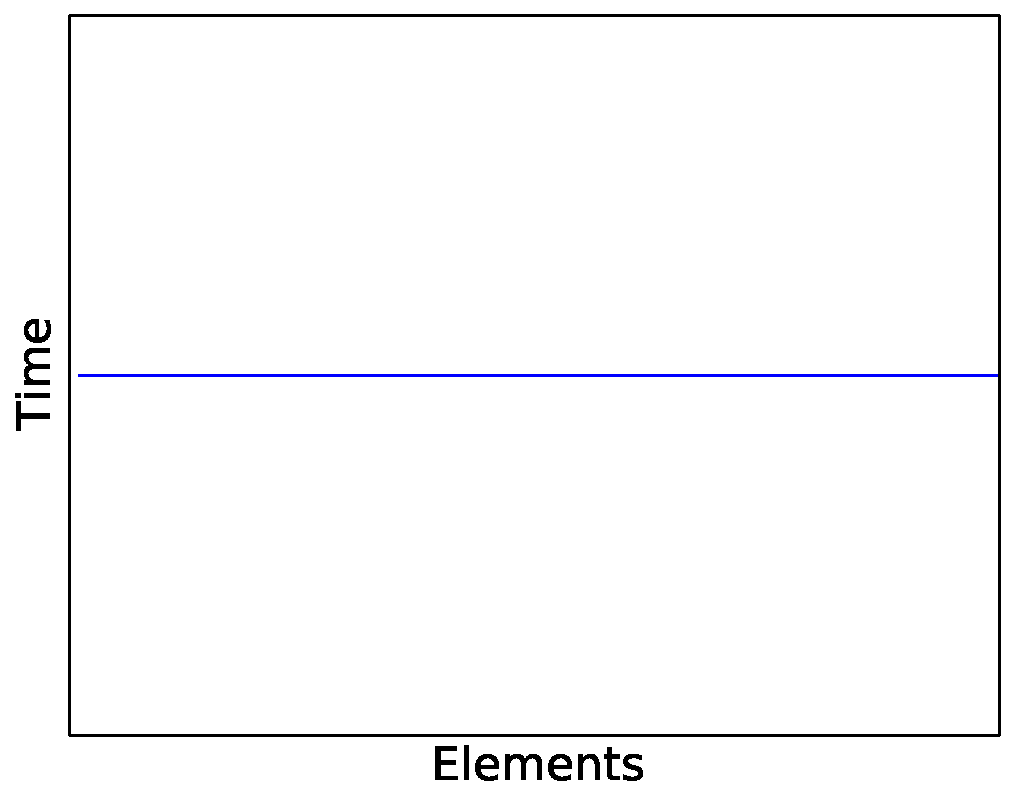
\includegraphics[width=\textwidth]{plot2_constant}
		\end{column}
		\begin{column}{0.55\textwidth}
			\begin{itemize}
				\item If there are no ``collisions'', look-up time is \textbf{constant} or $O(1)$ \pause
					\begin{itemize}
						\item (NB: constant \textbf{with respect to} $n$) \pause
					\end{itemize}
				\item I.e. doubling the size of the list \textbf{does not change} the look-up time \pause
				\item When there are collisions, need to fall back on something like linear or binary search within each bin
			\end{itemize}
		\end{column}
	\end{columns}
\end{frame}

\begin{frame}[fragile]{Don't reinvent the wheel!}
	\begin{itemize}
		\pause\item We are using search as an \textbf{example}, to learn the \textbf{principles} --- in practice
			you should hardly ever implement your own search
		\pause\item Linear search in C\#:
			\begin{itemize}
				\pause\item \lstinline{List<T>.IndexOf()}
			\end{itemize}
		\pause\item Binary search in C\#:
			\begin{itemize}
				\pause\item \lstinline{List<T>.BinarySearch()}
			\end{itemize}
		\pause\item Hash tables in C\#:
			\begin{itemize}
				\pause\item \lstinline{Dictionary<TKey, TValue>}
			\end{itemize}
	\end{itemize}
\end{frame}
